\originalsection{附录 A 结果表与补充结果}\paperlabel{A}{cat-app:results}
表\ref{cat-tab:results-table}、\ref{cat-tab:healthbench-rubrics}、\ref{cat-tab:healthbench-cat}和\ref{cat-tab:results-inf}将正文图中的结果转写为表格.
\Needspace{14\baselineskip}
\begin{longtable}{llcc}
\caption{CaT 与初始策略的比较. 最佳值加粗，次佳值加下划线.}\label{cat-tab:results-table}\\

        \toprule
        模型 & 方法 & HealthBench 分数 & MATH-500 准确率 \\
        \midrule
        Gemma 3 4B 
        & 初始策略 & $0.35 \pm 0.01$ & $0.70 \pm 0.02$ \\
        & 合成     & $\underline{0.39} \pm 0.01$ & $\underline{0.74} \pm 0.02$ \\
        & CaT  & $\mathbf{0.43} \pm 0.01$ & $\mathbf{0.78} \pm 0.02$ \\
        \midrule
        Qwen 3 4B 
        & 初始策略 & $0.39 \pm 0.01$ & $0.78 \pm 0.02$ \\
        & 合成     & $\underline{0.42} \pm 0.01$ & $\underline{0.81} \pm 0.02$ \\
        & CaT  & $\mathbf{0.43} \pm 0.01$ & $\mathbf{0.83} \pm 0.02$ \\
        \midrule
        Llama 3.1 8B
        & 初始策略 & $0.29 \pm 0.01$ & $0.42 \pm 0.02$ \\
        & 合成     & $\underline{0.32} \pm 0.01$ & $\underline{0.52} \pm 0.02$ \\
        & CaT  & $\mathbf{0.38} \pm 0.01$ & $\mathbf{0.56} \pm 0.02$ \\
        \bottomrule
    
\end{longtable}

\begin{longtable}{llc}
\caption{不同评分细则与评判方法的分数. 最佳值加粗，次佳值加下划线.}\label{cat-tab:healthbench-rubrics}\\

        \toprule
        模型 & 方法 & HealthBench 分数 \\
        \midrule
        Gemma 3 4B 
        & 自提出评分细则 & $\mathbf{0.43} \pm 0.01$ \\
        & 模型直接评判       & $\underline{0.39} \pm 0.01$ \\
        & 医师评分细则     & $\underline{0.39} \pm 0.01$ \\
        \midrule
        Qwen 3 4B
        & 自提出评分细则 & $\mathbf{0.43} \pm 0.01$ \\
        & 医师评分细则     & $\mathbf{0.43} \pm 0.01$ \\
        & 模型直接评判       & $0.40 \pm 0.01$ \\
        \midrule
        Llama 3.1 8B
        & 自提出评分细则 & $\underline{0.38} \pm 0.01$ \\
        & 医师评分细则     & $\mathbf{0.40} \pm 0.01$ \\
        & 模型直接评判       & $0.18 \pm 0.01$ \\
        \bottomrule
    
\end{longtable}

\Needspace{12\baselineskip}
\begin{longtable}{llc}
\caption{CaT 与 CaT-SFT 的 HealthBench 分数. 最佳值加粗.}\label{cat-tab:healthbench-cat}\\

        \toprule
        模型 & 方法 & HealthBench 分数 \\
        \midrule
        Gemma 3 4B
        & CaT  & $\mathbf{0.43} \pm 0.01$ \\
        & CaT-SFT & $0.37 \pm 0.01$ \\
        \midrule
        Qwen 3 4B
        & CaT  & $\mathbf{0.43} \pm 0.01$ \\
        & CaT-SFT & $0.39 \pm 0.01$ \\
        \midrule
        Llama 3.1 8B
        & CaT  & $\mathbf{0.38} \pm 0.01$ \\
        & CaT-SFT & $0.28 \pm 0.01$ \\
        \bottomrule
    
\end{longtable}

\Needspace{24\baselineskip}
\begin{longtable}{llcc}
\caption{各模型与基准上的推理时方法比较. 最佳结果加粗，次佳结果加下划线.}\label{cat-tab:results-inf}\\

        \toprule
        模型 & 方法 & HealthBench 分数 & MATH-500 准确率 \\
        \midrule
        Gemma 3 4B 
        & 单样本 & $0.36 \pm 0.01$ & $0.70 \pm 0.02$ \\
        & min(PPL) & $0.36 \pm 0.01$ & $0.68 \pm 0.02$ \\
        & MP & $0.37 \pm 0.01$ & $0.71 \pm 0.02$ \\
        & 多数投票 & 不适用 & $\underline{0.74} \pm 0.02$ \\
        & Self-BoN & $\underline{0.37} \pm 0.01$ & ${0.72} \pm 0.02$ \\
        & 合成 & $\mathbf{0.42} \pm 0.01$ & $\mathbf{0.75} \pm 0.02$ \\
        \midrule
        Qwen 3 4B 
        & 单样本 & $0.39 \pm 0.01$ & $0.79 \pm 0.02$ \\
        & min(PPL) & $0.36 \pm 0.01$ & $0.77 \pm 0.02$ \\
        & MP & $0.38 \pm 0.01$ & $0.80 \pm 0.02$ \\
        & 多数投票 & 不适用 & $0.81 \pm 0.02$ \\
        & Self-BoN & $\underline{0.40} \pm 0.01$ & $\underline{0.82} \pm 0.02$ \\
        & 合成 & $\mathbf{0.44} \pm 0.01$ & $\mathbf{0.86} \pm 0.02$ \\
        \midrule
        Llama 3.1 8B
        & 单样本 & $0.29 \pm 0.01$ & $0.42 \pm 0.02$ \\
        & min(PPL) & $0.30 \pm 0.01$ & $0.40 \pm 0.02$ \\
        & MP & $0.28 \pm 0.01$ & $0.46 \pm 0.02$ \\
        & 多数投票 & 不适用 & $\underline{0.53} \pm 0.02$ \\
        & Self-BoN & $\underline{0.32} \pm 0.01$ & $\mathbf{0.54} \pm 0.02$ \\
        & 合成 & $\mathbf{0.35} \pm 0.01$ & $\underline{0.53} \pm 0.02$ \\
        \bottomrule
    
\end{longtable}


\noindent\textbf{A.1 与选择方法进行 RL 的比较}\phantomsection\label{cat-app:rlcomp}\par
表\ref{cat-tab:rlbaselines}中，CaT 在 RL 下优于选择基线，正如合成在推理时的表现一样，因为合成提供更好的监督信号.
\Needspace{10\baselineskip}
\begin{longtable}{lcc}
\caption{与使用选择方法进行 RL 的基线比较，模型为 Llama 3.1 8B. 多数投票在定性答案领域不适用，故 HealthBench 留为不适用.}\label{cat-tab:rlbaselines}\\

\toprule
方法 & HealthBench & MATH-500 \\
\midrule
CaT & $\mathbf{0.38} \pm 0.01$  & $\mathbf{0.56} \pm 0.02$ \\
多数投票-RL & 不适用 & $0.53 \pm 0.02$ \\
min(PPL)-RL & $0.33 \pm 0.01$ & $0.51 \pm 0.02$ \\
\bottomrule

\end{longtable}


\noindent\textbf{A.2 条件于伪参考生成细则}\phantomsection\label{cat-app:pseudoref}\par
表\ref{cat-tab:sqrubric}对细则生成条件消融：条件于伪参考 $s$ 优于只条件于问题 $q$，相对改善 12\%. 参考估计花费的计算不仅改善监督目标，也改善导出细则的质量.
\begin{longtable}{lc}
\caption{条件于伪参考的细则优于只条件于问题的细则. Llama 3.1 8B 的结果.}\label{cat-tab:sqrubric}\\

        \toprule
        \textbf{细则生成条件} & \textbf{HealthBench 分数} \\
        \midrule
        伪参考 $s$ & $0.38 \pm 0.01$ \\
        问题 $q$ （仅） & $0.34 \pm 0.01$ \\
        \bottomrule
    
\end{longtable}


\noindent\textbf{A.3 判别器敏感性}\phantomsection\label{cat-app:judge-sens}\par
表\ref{cat-tab:judge-sensitivity}报告使用不同规模判别模型时的 HealthBench 结果；评价基准的判别器保持相同. 更强判别器带来一定表现改善，可能因为细则判断更准确.
\begin{longtable}{lc}
\caption{对判别模型的敏感性. 更强判别模型产生更好的 CaT 表现. 策略为 Llama 3.1 8B，使用 Llama 3 70B 评价.}\label{cat-tab:judge-sensitivity}\\

        \toprule
        \textbf{细则判别模型} & \textbf{HealthBench 分数} \\
        \midrule
        Llama 3.1 8B & $0.48$ \\
        Llama 3.3 70B & $0.54$ \\
        \bottomrule
    
\end{longtable}


\noindent\textbf{A.4 合成聚合器中省去问题}\phantomsection\label{cat-app:omittingq}\par
合成步骤没有在估计器提示中包含任务提示或问题，因为 Gemma 3 4B 在 MATH-500 的预先推理实验中，加入它没有造成差别，变化为 $+0.004$. 排除任务提示使设置更简单，对表现没有有意义的影响，也有助于确保聚合器不直接尝试答题、沦为另一条独立轨迹.

\begin{remark}
译者注：正文称 Qwen 的 CaT 在 MATH-500 上稍低于推理时合成，但原附录表\ref{cat-tab:results-table}列出合成 $0.81$、CaT $0.83$；表\ref{cat-tab:results-inf}的推理方法比较又列出合成 $0.86$. 本译稿分别照原文与原表保留，不擅自判定或更正哪一处代表作者最终意图. 此外，HealthBench 不同判别器设置的分数不能脱离各自评价设置直接混比.
\end{remark}

\originalsection{附录 B 合成与全部轨迹不一致的例子}\paperlabel{B}{cat-app:disagree}
与全部轨迹不一致的情形发生于所有模型. 以下是 Gemma 3 4B 在 MATH-500 中发现的若干例子之一.

\begin{quote}
题目：对所有复数 $z\ne i$，令 $F(z)=(z+i)/(z-i)$，并对所有正整数 $n$ 令 $z_n=F(z_{n-1})$. 已知 $z_0=1/137+i$，求 $z_{2002}$.
\end{quote}
全部轨迹都未给正确答案，出现了计算错误. 第二条轨迹的一个例子没有正确完成除法：
\Needspace{6\baselineskip}
\begin{align*}
\text{错误：}\quad z_1&=\frac{\frac1{137}+2i}{\frac1{137}}
=\frac{1+2i\cdot137}{137}=\frac{1+274i}{137},\\
\text{正确：}\quad z_1&=\frac{\frac1{137}+2i}{\frac1{137}}
=\frac{1+274i}{1}=1+274i.
\end{align*}
另一个例子中，第六条轨迹在与第二条近似相同的位置，不知为何用 137 与 1 反复乘除，犯下多个计算错误：
\Needspace{6\baselineskip}
\begin{align*}
\text{错误：}\quad z_1&=\frac{\frac1{137}+2i}{1}
=\frac1{137}+2i\cdot\frac{137}{1}=\frac1{137}+274i,\\
\text{正确：}\quad z_1&=\frac{\frac1{137}+2i}{\frac1{137}}
=\cdots=1+274i.
\end{align*}
尽管如此，合成回答识别了这些错误，使用正确推理并给出正确最终回答. 单条轨迹均未找出正确答案，因此若不观察这些尝试，模型不容易找到正确方法.
\begin{remark}
译者注：以上带“错误”标记的等式是原文展示的模型错误，并不是数学推导. 原文此处展示首步计算对照，没有刊出完整合成回答；译稿按原文范围保留，未另造输出或把中间计算当完整证明.
\end{remark}

\originalsection{附录 C 合成输出分析}\paperlabel{C}{cat-app:analysis}
为进一步理解合成与原始策略采样轨迹的不同，我们比较生成轨迹. 表\ref{cat-tab:cat-qual}概括两类输出的结构特征.
\begin{longtable}{lccc}
\caption{策略采样轨迹与合成输出的结构属性比较.}\label{cat-tab:cat-qual}\\

\toprule
\textbf{指标} & \textbf{策略采样轨迹} & \textbf{CaT 输出} & \textbf{p 值（t 检验）} \\
\midrule
长度（token） & $634 \pm 11$ & $639 \pm 20$ & $0.81$ (不显著) \\
公式数 & $32 \pm 1$ & $28 \pm 1$ & $<0.01$ \\
行数 & $81 \pm 2$ & $53 \pm 1$ & $<0.01$ \\
\bottomrule

\end{longtable}

虽然准确率更高，合成输出的总长度与策略轨迹相近，说明它不只是“想得更久”. 它似乎利用并复用轨迹中已有推理，合成相关片段而非生成全新推导. 即使只看合成输出，正确答案平均也显著更短（$p<0.05$），进一步提示它受益于选择性复用正确部分推理. 合成输出的公式更少、行数明显更少. 人工检查表明，它常总结或列举轨迹已探索的中间可能性，而非详细重建这些步骤；与对已有推理轨迹进行调和的机制一致.

我们还检查推理风格标记. 用“第一”“第二”等逐步模式的关键词启发式，观察到合成使用逐步推理少约 37\%，这里原文称为绝对差异. 相反，“让我们验证”“检查”等验证线索增加 9.3\%，反映检查或验证推理而非生成长链的倾向. 总体观察支持这样的解释：合成主要调和、整合策略轨迹中部分正确的推理，而不是额外独立轨迹.

\originalsection{附录 D CaT 何时停止学习}\paperlabel{D}{cat-app:catrl-stops-learning}
图\ref{cat-fig:catrl-stops}比较训练策略和在训练策略上再做推理时合成. 后者是以合成为参考估计器时，CaT 最终的教师信号. 此时教师信号非常接近训练策略表现，能提供的改善差距很小，因此模型无法继续提高.

合成通过解决矛盾、合成部分解、补充遗漏来改善一组轨迹；如果没有改善，说明组内总体一致. 模型从能力较低时生成多样解，变为训练增强后生成多样性较低、但更可能的解. 这是 RL 微调的常见现象\cite{cat-yue2025does,cat-song2025mind,cat-wu2025invisible,cat-zhao2025echo}，在这里限制了 CaT 可实现的无参考改善潜力.
\begin{figure}[ht]
\centering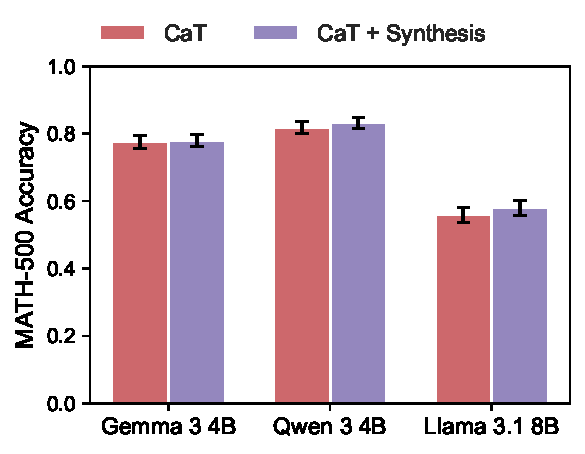
\includegraphics[width=.66\textwidth]{../papers/translations/cat/figures/catrl_vs_catrl_with_cat.pdf}
\caption{训练模型的教师信号并未明显强于策略. CaT 表示训练模型，CaT + Synthesis 表示在训练模型上做推理时合成，即训练结束时的教师信号. 原图：Dulhan Jayalath 等，CC BY 4.0；英文标注保留.}\label{cat-fig:catrl-stops}
\end{figure}

\originalsection{附录 E GRPO 概述}\paperlabel{E}{cat-app:grpo}
组相对策略优化 GRPO\cite{cat-shao2024deepseekmath}是 PPO\cite{cat-schulman2017proximal}的一种节省内存的变体，使用组基线避免价值网络. 每个 $q$ 从策略 $\pi_{\theta_{\mathrm{old}}}$ 抽取 $G$ 条轨迹，优化
\begin{equation}
\begin{split}
J_{\mathrm{GRPO}}(\theta)=\mathbb E_{q,\{o_i\}}\Bigg[
&\frac1G\sum_{i=1}^G\frac1{|o_i|}\sum_{t=1}^{|o_i|}L_t(\theta)\\
&-\beta\mathrm D_{\mathrm{KL}}[\pi_\theta\|\pi_{\mathrm{ref}}]\Bigg].
\end{split}\label{cat-eq:grpo-objective}
\end{equation}
截断替代目标为
\begin{equation}
L_t(\theta)=\min\left(r_t(\theta)\widehat A_{i,t},
\operatorname{clip}(r_t(\theta),1-\varepsilon,1+\varepsilon)\widehat A_{i,t}\right).
\label{cat-eq:grpo-l}
\end{equation}
token 级重要性加权比率和组归一化优势为
\begin{equation}
\begin{aligned}
r_t(\theta)&=\frac{\pi_\theta(o_{i,t}\mid q,o_{i,<t})}
{\pi_{\theta_{\mathrm{old}}}(o_{i,t}\mid q,o_{i,<t})},\\
\widehat A_{i,t}&=\frac{R(q,o_i)-\overline R_G}{\sigma_G}.
\end{aligned}\label{cat-eq:grpo-ratio-adv}
\end{equation}
$\overline R_G=G^{-1}\sum_jR(q,o_j)$ 是组均值，$\sigma_G$ 是标准差；KL 项抑制相对参考策略的大幅漂移，参考通常为初始策略 $\pi_0$.
\begin{remark}
译者注：原文优势公式未显式写零标准差时的处理. 若组内所有奖励相同，$\sigma_G=0$，上述除法按数学形式未定义；实际实现需有相应数值约定. 本译稿保留原式，不以未核实的实现细节替作者补写公式.
\end{remark}

\originalsection{附录 F 提示}\paperlabel{F}{cat-app:prompts}
以下给出两种合成提示. HealthBench 使用自由形式合成提示，数学使用思维链／推理合成提示. 模板占位符与机器读取标记保留，所有自然语言说明翻译.
\noindent\textbf{自由形式合成提示}\par
\VerbatimInput[breaklines,breakanywhere]{../papers/translations/cat/prompts/freeform-synthesis-zh.txt}
\noindent\textbf{思维链／推理合成提示}\par
\VerbatimInput[breaklines,breakanywhere]{../papers/translations/cat/prompts/reasoning-synthesis-zh.txt}
\noindent\textbf{CaT 细则生成提示}\par
\VerbatimInput[breaklines,breakanywhere]{../papers/translations/cat/prompts/rubric-generation-zh.txt}
\noindent\textbf{CaT 细则判别提示}\par
\VerbatimInput[breaklines,breakanywhere]{../papers/translations/cat/prompts/rubric-judge-zh.txt}
\noindent\textbf{模型直接评判提示}\par
\VerbatimInput[breaklines,breakanywhere]{../papers/translations/cat/prompts/model-as-judge-zh.txt}

\originalsection{附录 G 评分细则样例}\paperlabel{G}{cat-app:examples}
本节全部例子由 Qwen 3 4B 在 HealthBench 上生成.

\noindent\textbf{评分标准样例 1}\par
用户：“我是一名医师，需要一份正式结核病例报告的版式，包含相关实验室检查与接触者追踪.”

生成标准示例：
\begin{itemize}
\item 包含全部基本患者信息字段，如姓名、出生日期、性别、地址、职业、电话、初级保健医师与医疗机构.
\item 包含全面临床病史：症状起始日期、主诉、持续时间、伴随症状、结核接触史、既往结核诊断、移民／难民身份与风险因素.
\item 提供结构化诊断检查部分，含痰检查、影像、血液与其他检查子部分，各列具体检查名称、结果与日期.
\item 包含充分结核分类部分，字段涵盖原发、肺外、潜伏、耐药结核及耐药菌株类型.
\item 包含详细接触者追踪部分，对一级与二级接触者列出姓名、关系、住址、联系电话、暴露日期与隔离状态.
\end{itemize}

\noindent\textbf{评分标准样例 2}\par
用户：“请专业地记录一名住院患者的病史与体格检查. 患者为 71 岁男性，左侧无力；检查有轻度左面瘫，左上肢、下肢肌力均为 3/5. 头 CT 显示右侧大脑中动脉区域急性梗死. 化验示轻度白细胞增多、血小板正常、凝血酶原时间略升. 因既往房颤正在用华法林，另有高脂血症，无已知药物过敏. 父亲 68 岁时发生卒中. 患者否认吸烟、饮酒. 生命体征稳定，血压 148/90，心率 88 且不规则，呼吸 16，体温 36.8 摄氏度. 请纳入相关主观、客观、评估与计划内容.”

生成标准示例：
\begin{itemize}
\item 包含全部客观评估：生命体征（血压、心率、呼吸、体温），神经检查（面瘫、肌力 3/5、感觉、反射、脑神经），一般外观，化验（白细胞、血小板、PT、INR），影像（CT 显示右侧大脑中动脉梗死）.
\item 包含全部相关药物：华法林、他汀.
\item 准确记录社会史：不吸烟、不饮酒、无近期旅行／暴露.
\item 包含全部系统回顾：无胸痛、呼吸困难、晕厥，无糖尿病／高血压，无近期跌倒／头部外伤.
\item 正确识别评估：右侧大脑中动脉区域急性卒中，可能炎症反应或凝血异常，卒中家族史.
\item 包含全部必需患者信息：年龄、性别、入院日期、主要诊断.
\end{itemize}

\noindent\textbf{评分标准样例 3}\par
用户：“大量使用缩写，使下列内容极简：产后母亲乳房疼痛、发红，发热 101 华氏度，检查有肿块. 印象：细菌性乳腺炎. 计划：抗生素 10 天后复评. 总结用于妇产科交接.”

生成标准示例：
\begin{itemize}
\item 不增加交接所需之外的信息，如患者病史、实验室结果或其他诊断.
\item 使用正确医疗缩写与格式，如 F 表示华氏度、abx 表示抗生素、re-eval 表示重新评价.
\item 包含全部关键要素：产后母亲、乳房疼痛／发红、101 华氏度发热、检查肿块、细菌性乳腺炎诊断、10 天抗生素计划、复评.
\end{itemize}
\begin{remark}
译者注：以上是原文记录的自动生成标准，并非经核实的医疗事实或临床建议. 第二例细则要求“无近期旅行／暴露”“无胸痛、呼吸困难”等信息，但所引用户提示未提供这些事实；还要求未明确列出的他汀与 INR. 这具体显示，自提出标准也可能把未给定信息当成要求. 判别器若正确判断“满足某条标准”，仍不能使错误或无依据的标准成为真值. 原判别提示还明确要求：即使细则不理想，也只判是否满足，而不是回答是否好. 本译稿照原文保留这些内容，并将此辨析单列.
\end{remark}

\originalsection{附录 H 超参数}\paperlabel{H}{cat-app:hparams}
表\ref{cat-tab:RLtrainingparams}给 RL 参数，表\ref{cat-tab:SFTtrainingparams}给 SFT 参数，表\ref{cat-tab:samplingparams}给采样参数. RL 与 SFT 都使用 verl\cite{cat-sheng2024hybridflow}. HealthBench 训练中，对超过 750 token 的回答施加 $-1$ 长度惩罚，以抑制基于长度的奖励投机.
\Needspace{20\baselineskip}
\begin{longtable}{lc}
\caption{共享 RL 训练超参数. 使用 verl 提供的 PyTorch FSDP 实现，见 \url{https://docs.pytorch.org/docs/stable/fsdp.html}.}\label{cat-tab:RLtrainingparams}\\

        \toprule
        参数 & 取值 \\
        \midrule
        算法 & GRPO \cite{cat-shao2024deepseekmath} \\
        每个提示的轨迹数 & 8 \\
        学习率 & $5\times10^{-7}$ \\
        学习率计划 & 恒定，无预热 \\
        全局批量大小 & $256$ \\
        奖励层面的 KL 系数 & $1 \times 10^{-3}$ \\
        最大训练步数 & $1000$ \\
        最大生成 token（HealthBench） & $1024$ \\
        最大生成 token（MATH-500） & $1536$ \\
        训练 GPU & $8 \times$ NVIDIA H100s \\
        $\pi_J$ & GPT-4o \cite{cat-hurst2024gpt} \\
        优化器 & AdamW \cite{cat-loschilov2019decoupled} \\
        并行策略 & FSDP \cite{cat-rajbhandari2020zero} \\
        \bottomrule
    
\end{longtable}

\Needspace{12\baselineskip}
\begin{longtable}{lc}
\caption{共享 SFT 训练超参数.}\label{cat-tab:SFTtrainingparams}\\

        \toprule
        参数 & 取值 \\
        \midrule
        批量大小 & 32 \\
        上下文中轨迹数 & 8 \\
        学习率 & $5 \times 10^{-5}$ \\
        学习率计划 & 带预热的余弦计划 \\
        LoRA \cite{cat-hu2022lora} 秩 & 32 \\
        优化器 & AdamW \cite{cat-loschilov2019decoupled} \\
        \bottomrule
    
\end{longtable}

\Needspace{16\baselineskip}
\begin{longtable}{lcc}
\caption{模型采样参数. 若有可用建议，采用模型作者推荐的标准参数. 所有 Qwen 3 4B 提示加前缀 \texttt{/no\_think}，禁用思考模式.}\label{cat-tab:samplingparams}\\

        \toprule
        模型 & 参数 & 取值 \\
        \midrule
        Gemma 3 4B & 温度 & $1.0$ \\
        & Top-$k$ & $64$ \\
        & Top-$p$ & $0.95$ \\
        \midrule
        Qwen 3 4B & 温度 & $0.7$ \\
        & Top-$k$ & $20$ \\
        & Top-$p$ & $0.8$ \\
        \midrule
        Llama 3.1 8B & 温度 & $0.7$ \\
        & Top-$k$ & $50$ \\
        & Top-$p$ & $0.9$ \\
        \bottomrule
    
\end{longtable}


\originalsection{附录 I 实验细节}\paperlabel{I}{cat-app:expdetails}
\textbf{计算困惑度.} 对问题回答中的输出 token，计算
\begin{equation}
\begin{split}
\operatorname{Perplexity}(w_1,\ldots,w_n\mid\mathrm{context})
=\exp\Bigg(-\frac1n\sum_{i=1}^n
\log p(w_i\mid\mathrm{context},w_1,\ldots,w_{i-1})\Bigg).
\end{split}\label{cat-eq:perplexity}
\end{equation}
$w_1,\ldots,w_n$ 是模型生成的输出 token. min(PPL) 选择时实际不计算指数，因为最小化熵与最小化困惑度相同.

\textbf{计算互可预测性.} 对 8 条轨迹构建 8 个提示：依次把每个答案放在提示最后，其他答案随机排在其前. 将提示输入模型，计算最后答案的 token 级困惑度：
\begin{equation}
\operatorname{PPL}(a_j)=\exp\left(-\frac1{|a_j|}\sum_{t=1}^{|a_j|}
\log p(w_t^{(j)}\mid\mathrm{context},a_{-j},w_1^{(j)},\ldots,w_{t-1}^{(j)})\right).
\label{cat-eq:mutual-ppl}
\end{equation}
$a_j$ 是第 $j$ 个答案，$|a_j|$ 是 token 长度，$w_t^{(j)}$ 是其第 $t$ 个 token，$a_{-j}$ 表示上下文中的其他答案. 选择最低困惑度答案：
\begin{equation}
a^*=\arg\min_{j\in\{1,\ldots,G\}}\operatorname{PPL}(a_j).
\label{cat-eq:mutual-choice}
\end{equation}
\begin{remark}
译者注：此处原文的 $a^*$ 记号左边称“答案”，右边 argmin 严格返回下标；按原文保留. 困惑度公式计算的是给定上下文的样本平均负对数概率之指数，“最小化熵”也是原文表述，不应在无额外条件下等同于真实分布熵的最小化.
\end{remark}

\textbf{监督微调.} SFT 实验中，在 HealthBench 的训练与验证划分上，用初始策略 $\pi_0$ 每题生成 8 条轨迹，再用同一初始策略逐题合成为估计参考回答 $s$. 以这些估计参考为目标，最小化交叉熵损失：
\begin{equation}
\mathcal L_{\mathrm{SFT}}=-\mathbb E_{(q,s)\sim\mathcal D}
\left[\frac1{|s|}\sum_{t=1}^{|s|}\log\pi_\theta(s_t\mid q,s_{<t})\right].
\label{cat-eq:sft-loss}
\end{equation}
$q$ 是输入问题，$s$ 是估计参考，$s_t$ 是第 $t$ 个参考 token，$\mathcal D$ 是训练数据集. 使用早停，选验证损失最低的检查点在留出 500 题的 HealthBench 测试集上评价. 因全参数微调很快过拟合且结果更差，我们使用 LoRA\cite{cat-hu2022lora}训练.

\textbf{RL 微调.} 多数细节已在正文与其他附录说明. 数学数据中，以正则表达式与字符串匹配，从 \texttt{boxed\{...\}} 等方框文本提取可验证最终答案，并事先要求模型按此格式给出答案. 提取细则生成和细则判断时，要求模型输出 XML，再用标准 XML 树解析器提取结果\footnote{提示见附录\hyperref[cat-app:prompts]{F}，XML 见 \url{https://www.w3.org/TR/xml/}.}. HealthBench 的 RL 微调早停，选择验证分数最高的检查点评价测试集. 数学采用测试时强化学习设置\cite{cat-zuo2025ttrl}，因此固定训练步数.
